\documentclass{article}

\usepackage{graphicx}
\usepackage{tikz}
\usepackage{tikzsymbols}
\usetikzlibrary{calc,patterns,shapes.geometric}
\pagestyle{empty}
\usepackage[margin=0pt]{geometry}
\geometry{papersize={14in,12in}}

\def\centerarc[#1](#2)(#3:#4:#5){\draw[#1] ($(#2)+({#5*cos(#3)},{#5*sin(#3)})$) arc (#3:#4:#5);}

\begin{document}
	\begin{figure}
		\centering
		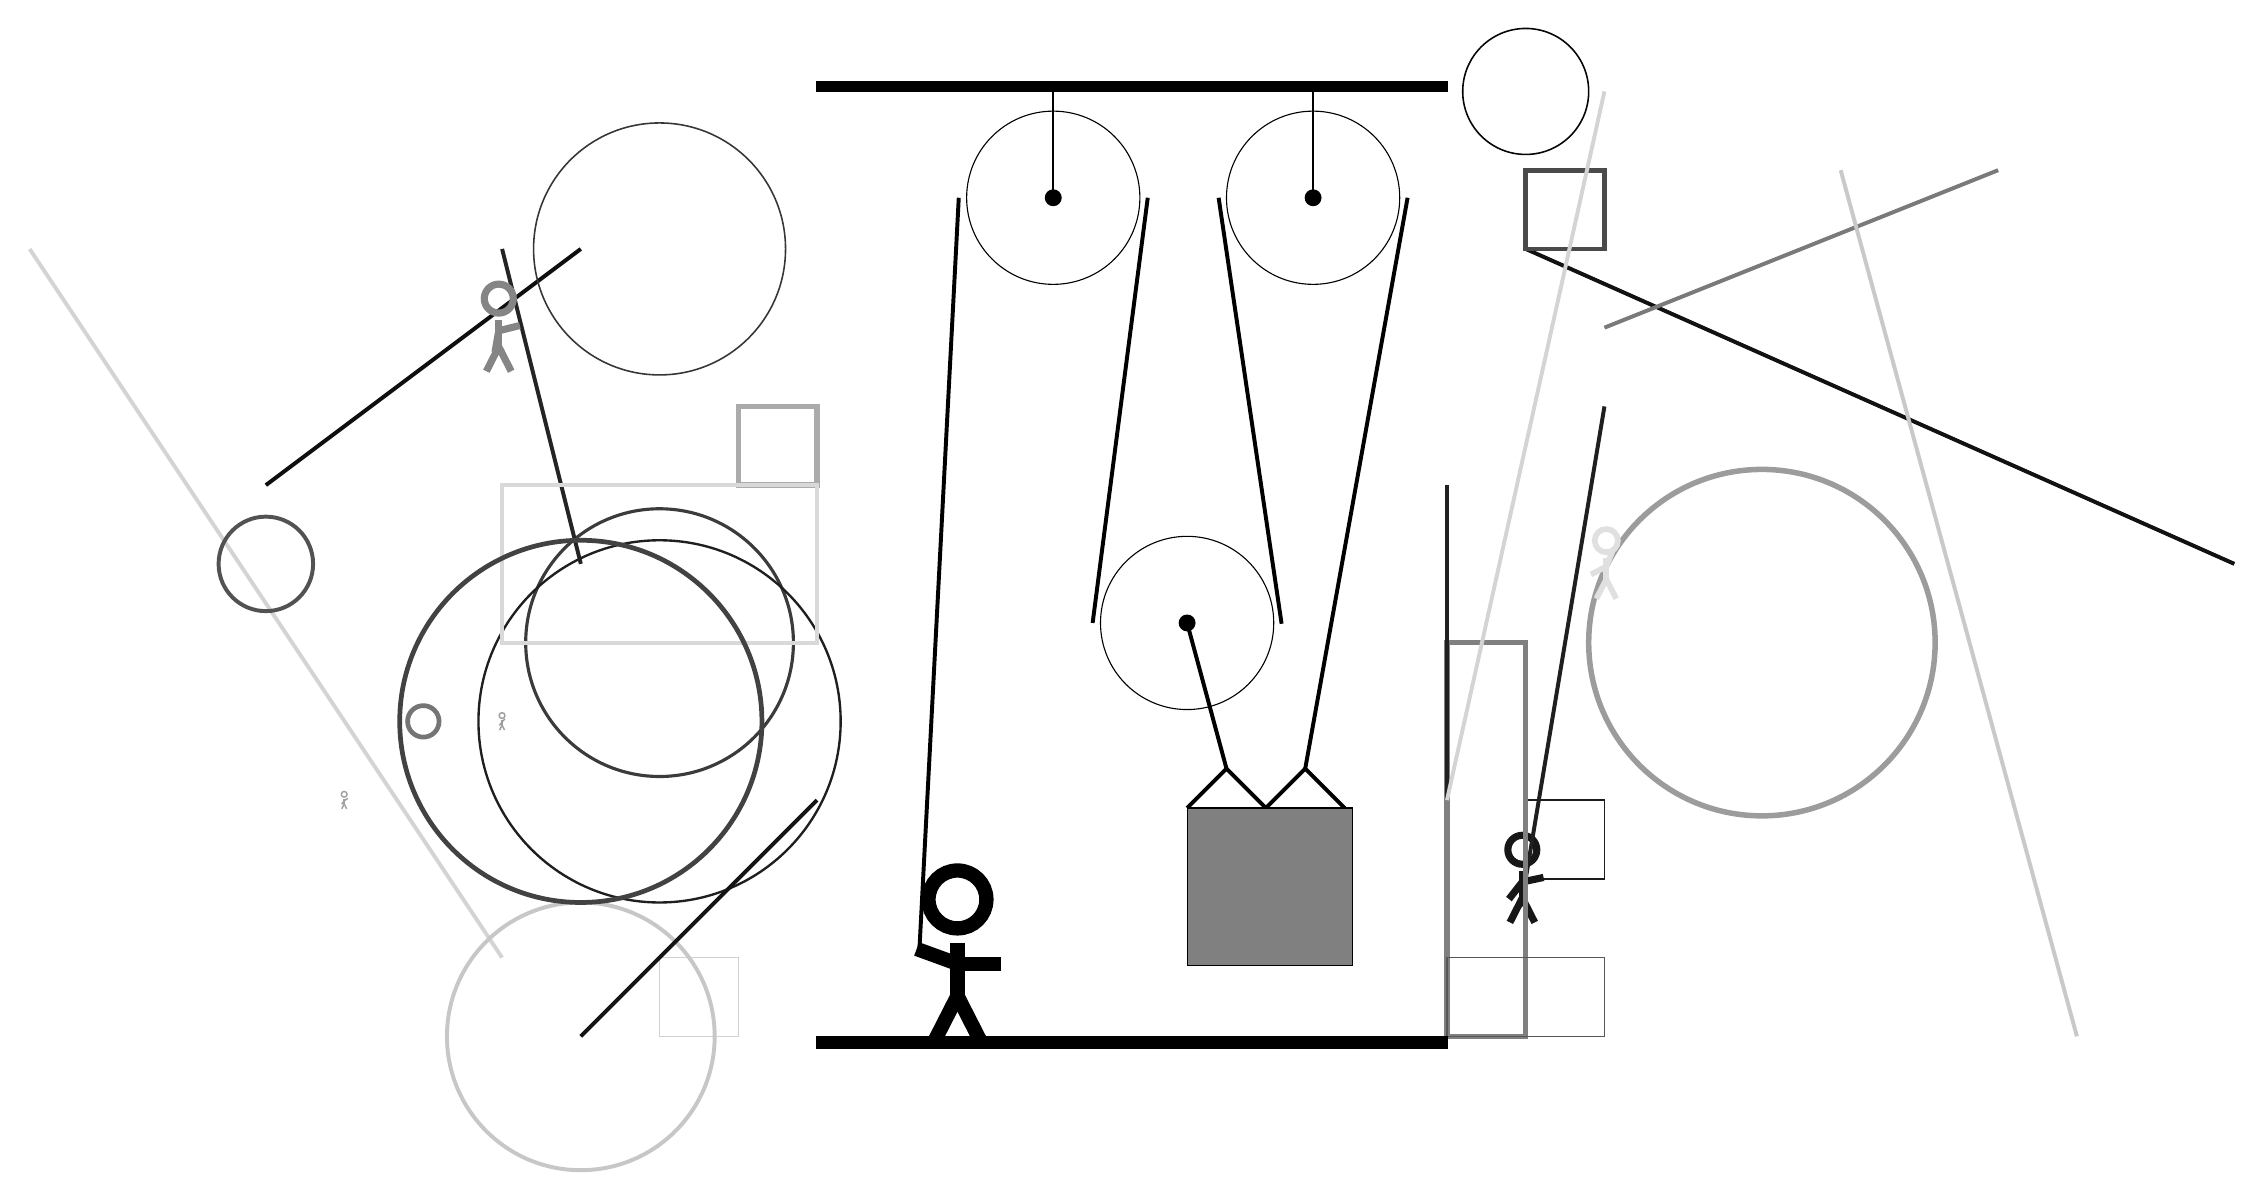
\begin{tikzpicture}
			%%%%% START %%%%%
			
			\draw[fill=black] (-2, 9) rectangle (6, 9.125);
			
			\draw (1, 7.65) circle (1.1);
			\draw[fill=black] (1, 7.65) circle (0.1);
			\draw[thick] (1, 7.65) -- (1, 9);
			
			\draw[line width=0.5mm, color=black!93](7, 7) -- (16, 3);
			
			\draw[line width=0.5mm, color=black!94](-5, 7) -- (-9, 4);
			\draw[line width=0.2mm, color=black!89] (7, -1) rectangle (8, 0);
			\draw [line width=0.4mm, color=black!77](-4, 2) circle (1.7);
			\draw[line width=0.6mm, color=black!71] (7, 8) rectangle (8, 7);
			\node[line width=0.7mm, color=black!37] at (-8, 0) {\Strichmaxerl[1][54][32]};
			
			\draw[line width=0.5mm, color=black!17](-6, -2) -- (-12, 7);
			\node[line width=0.6mm, color=black!91] at (7, -1) {\Strichmaxerl[5][52][12]};
			\draw[line width=0.2mm, color=black!18] (-3, -3) rectangle (-4, -2);
			\draw[line width=0.5mm, color=black!88](7, -1) -- (8, 5);
			
			\draw[line width=0.7mm, color=black!50] (7, 2) rectangle (6, -3);
			\draw[line width=0.2mm, color=black!66] (8, -2) rectangle (6, -3);
			\draw [line width=0.5mm, color=black!22](-5, -3) circle (1.7);
			
			\draw[line width=0.5mm, color=black!86](-5, 3) -- (-6, 7);
			\draw [line width=0.3mm, color=black!88](-4, 1) circle (2.3);
			\draw[line width=0.7mm, color=black!33] (-2, 4) rectangle (-3, 5);
			
			\draw[line width=0.5mm, color=black!15] (-2, 4) rectangle (-6, 2);
			
			\draw [line width=0.5mm, color=black!68](-9, 3) circle (0.6);
			\draw[line width=0.5mm, color=black!92](-2, 0) -- (-5, -3);
			
			\draw[line width=0.5mm, color=black!87](6, 4) -- (6, 0);
			\draw [line width=0.7mm, color=black!39](10, 2) circle (2.2);
			
			\node[line width=0.3mm, color=black!12] at (8, 3) {\Strichmaxerl[4][28][68]};
			\draw [line width=0.6mm, color=black!74](-5, 1) circle (2.3);
			\draw[line width=0.5mm, color=black!17](8, 9) -- (6, 0);
			\draw[line width=0.5mm, color=black!52](8, 6) -- (13, 8);
			\draw[line width=0.5mm, color=black!21](11, 8) -- (14, -3);
			\draw [line width=0.6mm, color=black!54](-7, 1) circle (0.2);
			\node[line width=0.4mm, color=black!38] at (-6, 1) {\Strichmaxerl[1][52][47]};
			\draw [line width=0.2mm, color=black!98](7, 9) circle (0.8);
			\node[line width=0.6mm, color=black!48] at (-6, 6) {\Strichmaxerl[5][80][14]};
			\draw [line width=0.2mm, color=black!79](-4, 7) circle (1.6);
			
			\draw (4.3, 7.65) circle (1.1);
			\draw[fill=black] (4.3, 7.65) circle (0.1);
			\draw[thick] (4.3, 7.65) -- (4.3, 9);
			
			\draw (2.7, 2.25) circle (1.1);
			\draw[fill=black] (2.7, 2.25) circle (0.1);
			
			\draw[line width=0.5mm]  (2.7, -0.1) -- (3.2, 0.4) -- (3.7, -0.1) -- (4.2, 0.4) -- (4.7, -0.1);
			\draw[fill=black!50] (2.7, -0.1) rectangle (4.8, -2.1);
			
			\draw[line width=0.5mm](-0.7, -1.9) -- (-0.2, 7.65);
			\centerarc[line width=0.5mm](1, 7.65)(0:180:1.2000000000000002);
			\draw[line width=0.5mm](2.2, 7.65) -- (1.5, 2.25);
			\centerarc[line width=0.5mm](2.7, 2.25)(180:370:1.2000000000000002);
			\draw[line width=0.5mm] (3.9, 2.24) -- (3.1, 7.65);
			\centerarc[line width=0.5mm](4.3, 7.65)(0:180:1.2000000000000002);
			\draw[line width=0.5mm](4.2, 0.4) -- (5.5, 7.65);
			\draw[line width=0.5mm] (3.2, 0.4) -- (2.7, 2.25);
			
			\node at (-0.2, -2) {\Strichmaxerl[10][-20][0]};
			
			\draw[fill=black] (-2, -3) rectangle (6, -3.15);
			
			%%%%% END %%%%%
		\end{tikzpicture}
	\end{figure}	
\end{document}